%\documentclass[letterpaper, 10 pt, conference]{ieeeconf} 
%\IEEEoverridecommandlockouts    
%\overrideIEEEmargins           
%\addtolength{\topmargin}{.1in}
% \addtolength{\textheight}{-.1in}
%\usepackage{cite}
\documentclass{article}
\usepackage{amsmath,amssymb,amsfonts}
\usepackage{graphicx}
\usepackage{xcolor, cancel}
\usepackage{placeins}
\newtheorem{theorem}{Theorem}
\newtheorem{lemma}{Lemma}
\newtheorem{definition}{Definition}
\newtheorem{note}{Note}
\newtheorem{property}{Property}

\newcommand{\norm}[1]{\left\|#1\right\|}
\newcommand{\abf}{\mathbf{a}}
\newcommand{\ebf}{\mathbf{e}}
\newcommand{\fbf}{\mathbf{f}}
\newcommand{\mbf}{\mathbf{m}}
\newcommand{\pbf}{\mathbf{p}}
\newcommand{\ubf}{\mathbf{u}}
\newcommand{\vbf}{\mathbf{v}}
\newcommand{\xbf}{\mathbf{x}}
\newcommand{\ybf}{\mathbf{y}}
\newcommand{\zbf}{\mathbf{z}}
\newcommand{\Jbf}{\mathbf{J}}
\newcommand{\Mbf}{\mathbf{M}}
\newcommand{\deltabf}{\boldsymbol{\delta}}
\newcommand{\ellbf}{\boldsymbol{\ell}}
\newcommand{\omegabf}{\boldsymbol{\omega}}
\newcommand{\taubf}{\boldsymbol{\tau}}
\newcommand{\rwb}[1]{{\color{blue}#1}}
\newcommand{\landon}[1]{{\color{orange}#1}}
\renewcommand\CancelColor{\color{orange}}


\title{Hypersonic Vehicle Simulation}
\author{
    Randal W. Beard
    \thanks{
        This work has been funded by....
    }
    \thanks{
        R. W. Beard is with the Electrical and Computer Engineering Department at Brigham Young University, Provo, UT, 84602 USA.  (e-mail: beard@byu.edu)
    }
}
\date{\today}

\begin{document}

\maketitle
\thispagestyle{empty}

    \begin{abstract}
        Cool stuff in this paper.
    \end{abstract}

%-------------------------------------------------------
\section{Introduction}

%-------------------------------------------------------
\section{Animation}

%-------------------------------------------------------
\section{Dynamics}
The dynamics are adapted from the equations given in~\cite{LiZhangZhang23}.

Let $\pbf_m^i\in\mathbb{R}^3$ be the position of the missile expressed in the inertial North-East-Down (NED) frame, and $\pbf_t^i\in\mathbb{R}^3$ be the inertial position of the target in the NED frame.  Define the body frame of the hypersonic vehicle as the $\xbf_b$-axis pointing out the nose of the vehicle, the $\zbf_b$-axis pointing toward the belly of the hypersonic vehicle, and the $\ybf_b$-axis such that $(\xbf_b,\ybf_b,\zbf_b)$ form a right handed coordinate system.  Let $R_b^i\in SO(3)$ represent the attitude of the body relative to the inertial frame, i.e.,
\[
R_b^i = \begin{pmatrix} \xbf_b^i & \ybf_b^i & \zbf_b^i \end{pmatrix}.
\]
Let $\vbf_m^b\in\mathbb{R}^3$ be the velocity of the missile expressed in the body frame, and let $\omegabf_m^b\mathbb{R}^3$ be the angular velocity of the missile expressed in the body frame.  Let $\deltabf\in\mathbb{R}^3$ be the three rudder flaps that actuate the body frame along the $x$, $y$, and $z$ axes.  

Let $\Jbf=\text{diag}([J_x, J_y, J_z])$ be the inertia matrix of the missile, where $\text{diag}(\ubf)$ is the diagonal matrix with diagonal elements given by $\ubf$, then the missile dynamics are given by
	\begin{align*}
		\dot{\pbf}_m^i &= R_b^i \vbf_m^b \\
		\dot{\vbf}_m^b &= \vbf_m^b \times \omegabf_m^b + \frac{1}{m}\fbf\\
		\dot{R}_b^i &= R_b^i (\omegabf_m^b)^\wedge \\
		\dot{\omegabf}_m^b &= \Jbf^{-1}\left(-\omegabf_m^b \times \Jbf\omegabf_m^b + \Mbf \right)  
	\end{align*}
where
	\[
		\begin{pmatrix} a \\ b \\ c \end{pmatrix}^\wedge \triangleq \begin{pmatrix} 0 & -c & b \\ c & 0 & -a \\ -b & a & 0 \end{pmatrix}.
	\]
Assuming the absence of wind, then $V_a=\norm{\vbf_m^b}$ is the airspeed and the angle-of-attack $\alpha$ and the side-slip $\beta$ are given by
\begin{align}
\alpha &= \text{atan2}(\vbf_m^b\cdot \ebf_3, \vbf_m^b\cdot\ebf_1) \\
\beta &= \sin^{-1}\left(\frac{\vbf_m^b\cdot \ebf_2}{V_a}\right),	
\end{align}
where
\[
\ebf_1 = (1, 0, 0)^\top, \qquad \ebf_2 = (0, 1, 0)^\top, \qquad \ebf_3 = (0, 0, 1)^\top.
\]
The force and torque models are given by
\begin{align*}
	\fbf &= \frac{1}{2}\rho V_a^2 S\left(\fbf_\alpha\alpha + \fbf_\beta \beta\right) \\
	\Mbf &= \frac{1}{2}\rho V_a^2 S L \left(\mbf_\alpha\alpha + \mbf_\beta\beta + \text{diag}(\mbf_\delta)\deltabf \right),
\end{align*}
where the rudder dynamics are given by
\[
	\dot{\deltabf} = \text{diag}(\taubf)^{-1}(\deltabf^c - \deltabf),
\]
with $\deltabf^c$ being the commanded rudder angles, 
and where 
\begin{align*}
	\fbf_\alpha &= \begin{pmatrix} 0, & 0, & c_z^\alpha \end{pmatrix}^\top\\ 
	\fbf_\beta &= \begin{pmatrix} 0, & c_y^\beta, & 0\end{pmatrix}^\top \\
	\mbf_\alpha &= \begin{pmatrix} m_x^\alpha, & m_y^\alpha, & 0 \end{pmatrix}^\top \\
	\qquad
	\mbf_\beta &= \begin{pmatrix} m_x^\beta, & 0, & m_z^\beta \end{pmatrix}^\top \\
	\qquad
	\mbf_\delta &= \begin{pmatrix} m_x^\delta, & m_y^\delta, & m_z^\delta \end{pmatrix}^\top \\
	\taubf &= \begin{pmatrix}\tau_x, & \tau_y, & \tau_z \end{pmatrix}^\top.
\end{align*}

The parameters listed in~\cite{LiZhangZhang23} are given in Table~\ref{tab:parameters}. 
\begin{table}[h!]
\caption{Parameters for hypersonic vehicle.}
\centering
 \begin{tabular}{||c c || c c||} 
 \hline
 Parameter & Value & Parameter & Value \\ [0.5ex] 
 \hline\hline
 $m$ & $1200~kg$ & $c_z^\alpha$ & $-57.15$ \\ 
 $J_x$ & $100~kg\cdot m^2$ & $c_y^\beta$ & $-56.32$ \\
 $J_y$ & $5700~kg\cdot m^2$ & $m_x^\alpha$ & $0.45$ \\
 $J_z$ & $5800~kg\cdot m^2$ & $m_y^\alpha$ & $-28.15$ \\
 $\rho$ & $1.1558~kg/m^3$ & $m_x^\beta$ & $-0.38$ \\
 $S$ & $0.43~m^2$ & $m_z^\beta$ & $27.3$ \\
 $L$ & $0.6~m$ & $m_x^\delta$ & $2.13$ \\
 $\tau_x$, $\tau_y$, $\tau_z$ & $0.1~s$ & $m_z^\delta$ & $-26.6$ \\
  &  & $m_y^\delta$ & $-27.9$ \\ 
  &  & $c_z^\beta$ & $0.081$\\
  &  & $c_z^{\delta_y}$ & $-5.75$\\
  &  & $c_y^\alpha$ & $0.091$\\
  &  & $c_y^{\delta_z}$ & $5.6$\\[1ex] 
 \hline
 \end{tabular}
 \label{tab:parameters}
\end{table}

We will assume that the initial speed is $V_{a0} = 2000~m/s$. 



%-------------------------------------------------------
\section{Engagement Geometry}

\begin{figure}[htb]
  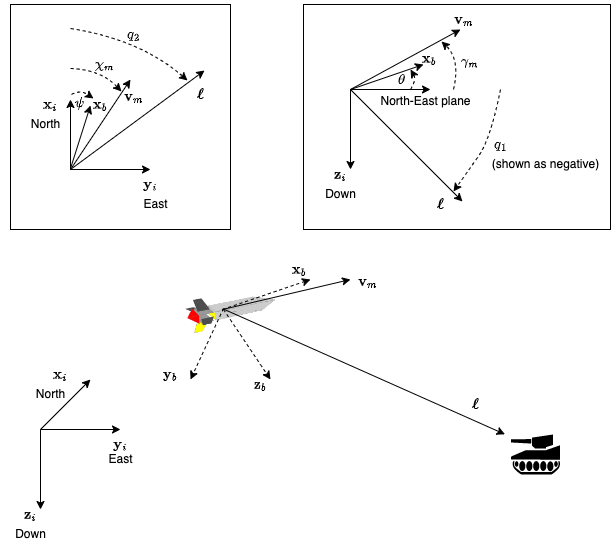
\includegraphics[width=0.90\linewidth]{./figures/los_geometry.png}
  \caption{The engagement geometry.  $\{\xbf_i, \ybf_i, \zbf_i\}$ is the inertial frame, $\{\xbf_b, \ybf_b, \zbf_b\}$ is the body frame with yaw angle $\psi$ and pitch angle $\theta$.  The velocity of the hypersonic vehicle is denoted $\vbf_M$ with azimuth $\psi_M$ and elevation $\theta_M$ angles measured relative to the inertial frame.  The line-of-sight vector from the hypersonic vehicle to the target is denoted $\boldsymbol{\ell}$ with azimuth and elevation angle denoted as $q_2$ and $q_1$ respectively.}
  \label{fig:los_geometry}
\end{figure}

The engagement geometry is shown in Figure~\ref{fig:los_geometry}.  If the position of the target is given by
$\pbf_t$, then the line-of-sight vector is given by
\[
\ellbf\triangleq \pbf_t - \pbf_m.
\]
We assume that the line-of-sight vector is measured in the body frame, and then internally resolved in the inertial frame.  The range to the target is given by
\[
r = \norm{\ellbf},
\]
and, as shown in Figure~\ref{fig:los_geometry}, the elevation and azimuth angles of $\boldsymbol{\ell}$ are given respectively by
\begin{align*}
	q_1 &= -\sin^{-1}\left(\frac{\ellbf^i_z}{\sqrt{\ellbf^{i2}_x+\ellbf^{i2}_y}}\right)\\
	q_2 &= \text{atan2}(\ell^i_y, \ellbf^i_x).
\end{align*}


The rotation angle from the line-of-sight (los) frame to the inertial frame is given by
\begin{align*}
R_\ell^i &= R_z(q_2)R_y(q_1) \\ 
		&= \begin{pmatrix}\cos q_2 & -\sin q_2 & 0 \\ \sin q_2 & \cos q_2 & 0 \\ 0 & 0 & 1 \end{pmatrix}
		   \begin{pmatrix}\cos q_1 & 0 & \sin q_1 \\ 0 & 1 & 0 \\ -\sin q_1 & 0 & \cos q_1 \end{pmatrix} \\
		 &= \begin{pmatrix} \cos q_1 \cos q_2 & -\sin q_2 & \sin q_1\cos q_2 \\ \cos q_1 \sin q_2 & \cos q_2 & \sin q_1 \sin q_2 \\ -\sin q_1 & 0 & \cos q_1 \end{pmatrix}
\end{align*}
Therefore, the light-of-sight vector in the inertial frame is given by
\begin{align*}
\ellbf^i &= \begin{pmatrix} \cos q_1 \cos q_2 & -\sin q_2 & \sin q_1\cos q_2 \\ \cos q_1 \sin q_2 & \cos q_2 & \sin q_1 \sin q_2 \\ -\sin q_1 & 0 & \cos q_1 \end{pmatrix}
		   \begin{pmatrix} r \\ 0 \\ 0 \end{pmatrix} \\
		 &= \begin{pmatrix} r\cos q_1 \cos q_2 \\ r \cos q_1 \sin q_2 \\ - r\sin q_1 \end{pmatrix}.
\end{align*}

%Given that
%\[
%\dot{R}_\ell^i = \omegabf_{\ell/i}^{i\wedge} R_\ell^i ,
%\]
%we get that the angular velocity of line-of-sight vector in the inertial frame is
%\begin{align*}
%	\omegabf_{\ell/i}^i &= (\dot{R}_\ell^i R_\ell^{i\top})^\vee \\
%	&= \left(\dot{q}_2 R_z^{'} R_y R_y^\top R_z^\top + \dot{q}_1 R_zR_y^{'} R_y^\top R_z^\top\right)^\vee \\
%	&= \left(\dot{q}_2 R_z^{'} R_z^\top + \dot{q}_1 R_zR_y^{'} R_y^\top R_z^\top\right)^\vee \\
%	&= \left(\dot{q}_2 \begin{pmatrix}0&-1&0\\1&0&0\\0&0&0\end{pmatrix} + \dot{q}_1 R_z\begin{pmatrix}0&0&1\\0&0&0\\-1&0&0\end{pmatrix} R_z^\top\right)^\vee \\
%	&= \begin{pmatrix}0 & -\dot{q}_2 & \dot{q}_1\cos q_2 \\
%						    \dot{q}_2 & 0 & \dot{q}_1\sin q_2 \\
%						    -\dot{q}_1\cos q_2 & -\dot{q}_1\sin q_2 & 0\end{pmatrix}^\vee \\
%\implies \omegabf_{\ell/i}^i &= \begin{pmatrix} -\dot{q}_1\sin q_2 \\ \dot{q}_1\cos q_2 \\ \dot{q}_2 \end{pmatrix}.
%\end{align*}

Given that
\[
\dot{R}_\ell^i = R_\ell^i \omegabf_{\ell/i}^{\ell \wedge}  ,
\]
we get that the angular velocity of line-of-sight vector in the line-of-sight frame is
\begin{align*}
	\omegabf_{\ell/i}^\ell &= (R_\ell^{i\top} \dot{R}_\ell^i )^\vee \\
	&= \left(\dot{q}_1 R_y^\top R_z^\top R_z R_y^{'} + \dot{q}_2 R_y^\top R_z^\top R_z^{'} R_y \right)^\vee \\
	&= \left(\dot{q}_1 R_y^\top R_y^{'} + \dot{q}_2 R_y^\top R_z^\top R_z^{'} R_y \right)^\vee \\
	&= \left(\dot{q}_1 \begin{pmatrix}0&0&1\\0&0&0\\-1&0&0\end{pmatrix} + \dot{q}_2 R_y^\top \begin{pmatrix}0&-1&0\\1&0&0\\0&0&0\end{pmatrix}R_y \right)^\vee \\
	&= \begin{pmatrix}
		0 & -\dot{q}_2\cos q_1 & \dot{q}_1 \\
		\dot{q}_2\cos q_1 & 0 & \dot{q}_2\sin q_1 \\
		-\dot{q}_1 & -\dot{q}_2\sin q_1 & 0
	   \end{pmatrix}^\vee \\
\implies \omegabf_{\ell/i}^\ell &= \begin{pmatrix} -\dot{q}_2\sin q_1 \\ \dot{q}_1 \\ \dot{q}_2\cos q_1 \end{pmatrix}.
\end{align*}


The velocity of the line-of-sight vector expressed in the line-of-sight frame is therefore 
\begin{align*}
	\vbf_{\ell/i}^\ell &= \frac{d}{dt}\ellbf^\ell + 	\omegabf_{\ell/i}^{\ell} \times \ellbf^\ell \\
	&= \begin{pmatrix} \dot{r} \\ 0 \\ 0 \end{pmatrix} + \begin{pmatrix}
		0 & -\dot{q}_2\cos q_1 & \dot{q}_1 \\
		\dot{q}_2\cos q_1 & 0 & \dot{q}_2\sin q_1 \\
		-\dot{q}_1 & -\dot{q}_2\sin q_1 & 0
	   \end{pmatrix} \begin{pmatrix}r \\ 0 \\ 0 \end{pmatrix} \\
	&= \begin{pmatrix}
 	    \dot{r} \\
 	    r\dot{q}_2  \cos q_1 \\
 	    -r \dot{q}_1 
 	   \end{pmatrix}.
\end{align*}
Similarly, the acceleration of the line-of-sight vector expressed in the line-of-sight frame is 
\begin{align*}
	\abf_{\ell/i}^\ell &= \frac{d}{dt}\vbf_{\ell/i}^\ell + 	\omegabf_{\ell/i}^{\ell} \times \vbf_{\ell/i}^\ell \\
	&= \begin{pmatrix} 
			\ddot{r} \\ 
			\dot{r}\dot{q}_2  \cos q_1 + r\ddot{q}_2\cos q_1 - r\dot{q}_2\dot{q_1}\sin q_1 \\ 
			-\dot{r} \dot{q}_1 - r\ddot{q}_1 
		\end{pmatrix} 
		+ \begin{pmatrix}
			0 & -\dot{q}_2\cos q_1 & \dot{q}_1 \\
			\dot{q}_2\cos q_1 & 0 & \dot{q}_2\sin q_1 \\
			-\dot{q}_1 & -\dot{q}_2\sin q_1 & 0
	   	  \end{pmatrix} 
	   	  \begin{pmatrix}
	   	  		\dot{r} \\
 	    		r\dot{q}_2  \cos q_1 \\
 	    		-r \dot{q}_1 
 	      \end{pmatrix} \\
	&= \begin{pmatrix}
 	    \ddot{r} - r\dot{q}_2^2\cos^2 q_1 -r\dot{q}_1^2 \\
 	     r\ddot{q}_2\cos q_1 + 2\dot{r}\dot{q}_2  \cos q_1  - 2r\dot{q}_1\dot{q}_2\sin q_1 \\
 	    - r\ddot{q}_1 -2\dot{r} \dot{q}_1  - r\dot{q}_2^2\cos q_1 \sin q_1 
 	   \end{pmatrix} \\
 	&= \begin{pmatrix}
 	    1 & 0 & 0 \\
 	    0 & 0 & r\cos q_1 \\
 	    0 & -r & 0  
 	   \end{pmatrix} \begin{pmatrix} \ddot{r} \\ \ddot{q}_1 \\ \ddot{q}_2 \end{pmatrix} 
 	   + \begin{pmatrix}
 	    - r\dot{q}_2^2\cos^2 q_1 -r\dot{q}_1^2 \\
 	     2\dot{r}\dot{q}_2  \cos q_1  - 2r\dot{q}_1\dot{q}_2\sin q_1 \\
 	    -2\dot{r} \dot{q}_1  - r\dot{q}_2^2\cos q_1 \sin q_1 
 	   \end{pmatrix}
\end{align*}

We also know that the acceleration of the line-of-sight vector is the acceleration of the target minus the acceleration of the hypersonic vehicle, therefore
\[
\abf_{\ell/i}^\ell = \abf_{t/i}^\ell - \abf_{m/i}^\ell,
\]
which implies that
\begin{align*}
	\begin{pmatrix} \ddot{r} \\ \ddot{q}_1 \\ \ddot{q}_2 \end{pmatrix} 
		&= \begin{pmatrix}
 	    1 & 0 & 0 \\
 	    0 & 0 & r\cos q_1 \\
 	    0 & -r & 0  
 	   \end{pmatrix}^{-1}\left(
 	   -\begin{pmatrix}
 	    - r\dot{q}_2^2\cos^2 q_1 -r\dot{q}_1^2 \\
 	     2\dot{r}\dot{q}_2  \cos q_1  - 2r\dot{q}_1\dot{q}_2\sin q_1 \\
 	    -2\dot{r} \dot{q}_1  - r\dot{q}_2^2\cos q_1 \sin q_1 
 	   \end{pmatrix} + \abf_{t/i}^\ell - \abf_{m/i}^\ell \right) \\
 	   &= \begin{pmatrix}
 	    1 & 0 & 0 \\
 	    0 & 0 & \frac{-1}{r} \\
 	    0 & \frac{1}{r\cos q_1} & 0  
 	   \end{pmatrix}\left(
 	   -\begin{pmatrix}
 	    - r\dot{q}_2^2\cos^2 q_1 -r\dot{q}_1^2 \\
 	     2\dot{r}\dot{q}_2  \cos q_1  - 2r\dot{q}_1\dot{q}_2\sin q_1 \\
 	    -2\dot{r} \dot{q}_1  - r\dot{q}_2^2\cos q_1 \sin q_1 
 	   \end{pmatrix} + \abf_{t/i}^\ell - \abf_{m/i}^\ell \right) \\
 	   &= \begin{pmatrix}
 	    	 r\dot{q}_2^2\cos^2 q_1 + r\dot{q}_1^2 \\
 	    	-2\frac{\dot{r}}{r} \dot{q}_1  - \dot{q}_2^2\cos q_1 \sin q_1 \\
 	     -2\frac{\dot{r}}{r} \dot{q}_2  + 2\dot{q}_1\dot{q}_2\tan q_1
 	   \end{pmatrix} 
 	   + \begin{pmatrix}
 	    1 & 0 & 0 \\
 	    0 & 0 & \frac{-1}{r} \\
 	    0 & \frac{1}{r\cos q_1} & 0  
 	   \end{pmatrix}\left(\abf_{t/i}^\ell - \abf_{m/i}^\ell \right) \\
\end{align*}

We can also write a force balance equation for the hypersonic vehicle to describe how the force impact the inertial flight path and course angles.
As shown in Figure~\ref{fig:los_geometry}, the velocity vector of the hypersonic vehicle expressed in the inertial frame is given by $\vbf_m^i$, which implies that that flight path angle and course angle are given by
\begin{align*}
	\gamma_m &= -\sin^{-1}\left(\frac{\vbf_{mz}^i}{\sqrt{\vbf_{mx}^{i2}+\vbf_{my}^{i2}}}\right)\\
	\chi_m &= \text{atan2}(\vbf_{my}^i, \vbf_{mx}^i).
\end{align*}
If $V_m=\norm{\vbf_{m/i}^i}$ is the magnitude of the velocity, then we can write
\[
\vbf_{m/i}^i = \begin{pmatrix} V_m \cos\chi_m \cos\gamma_m \\ V_m\sin\chi_m\cos\gamma_m \\ -V_m\sin\gamma_m \end{pmatrix}.
\]



which implies that
\begin{align*}
	\vbf_{m/i}^\ell &= R_i^\ell	\vbf_{m/i}^i \\
				    &= \begin{pmatrix} 
				    			\cos q_1 \cos q_2 & \cos q_1 \sin q_2 & -\sin q_1 \\ 
				    			-\sin q_2 & \cos q_2 & 0 \\ 
				    			\sin q_1\cos q_2 & \sin q_1 \sin q_2 & \cos q_1 \end{pmatrix}
				    		\begin{pmatrix} V_m \cos\chi_m \cos\gamma_m \\ V_m\sin\chi_m\cos\gamma_m \\ -V_m\sin\gamma_m \end{pmatrix} \\
				    &= V_m \begin{pmatrix}
 						 		\cos q_1 \cos\gamma_m \cos(q_2-\chi_m) + \sin q_1 \sin\gamma_m \\
 						 		-\cos\gamma_m \sin(q_2-\chi_m) \\
 						 		\sin q_1 \cos\gamma_m \cos(q_2-\chi_m) - \cos q_1 \sin\gamma_m 
 					       \end{pmatrix}
\end{align*}
Therefore
\begin{align*}
	\abf_{m/i}^\ell &= \frac{d}{dt}	\vbf_{m/i}^\ell + \omegabf_{\ell/i}^{\ell\wedge} \vbf_{m/i}^\ell \\
					&= \frac{d}{dt}	R_\ell^{i\top}	\vbf_{m/i}^i + R_\ell^{i\top}\dot{R}_\ell^i R_\ell^{i\top}	\vbf_{m/i}^i \\
					&= -	R_\ell^{i\top}\dot{R}_\ell^i R_\ell^{i\top} \vbf_{m/i}^i + R_\ell^{i\top} \dot{\vbf}_{m/i}^i + R_\ell^{i\top}\dot{R}_\ell^i R_\ell^{i\top} \vbf_{m/i}^i \\
					&= R_\ell^{i\top} \dot{\vbf}_{m/i}^i \\
					&= V_m R_\ell^{i\top}
				    		\begin{pmatrix}
				    			-\sin\chi_m \cos\gamma_m & -\cos\chi_m\sin\gamma_m \\ 
				    			\cos\chi_m\cos\gamma_m & -\sin\chi_m\sin\gamma_m \\ 
				    			0 & -\cos\gamma_m	
				    		\end{pmatrix}
				    		\begin{pmatrix}
				    			\dot{\chi}_m \\ \dot{\gamma}_m 
				    		\end{pmatrix},
\end{align*}
where we have assumed that $\dot{V}_m=0$.





	\begin{figure}[hhhh]
  		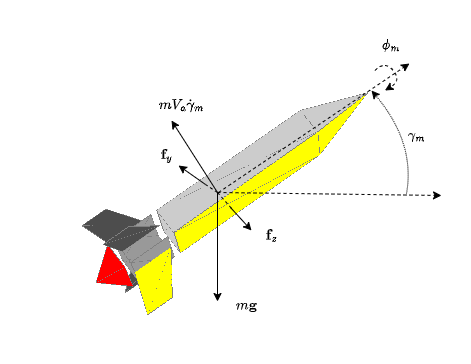
\includegraphics[width=0.49\linewidth]{./figures/vehicle_forces_longitudinal.png}
  		\caption{The longitudinal forces acting on the hypersonic vehicle when the flight path angle $\gamma_m$ is changing.}
        \label{fig:vehicle_forces_longitudinal}
  	\end{figure} 	
The longitudinal forces acting on the hypersonic vehicle are shown in Figure~\ref{fig:vehicle_forces_longitudinal}.  Summing the forces along the longitudinal axis gives
\[
mV_m \dot{\gamma}_m = mg\cos\gamma + f_z\cos\phi + f_y\sin\phi,
\]
from which we obtain
\[
\dot{\gamma}_m = \frac{g}{V_m}\cos\gamma + \frac{f_z\cos\phi + f_y\sin\phi}{mV_m}.
\]

	\begin{figure}[hhhh]
  		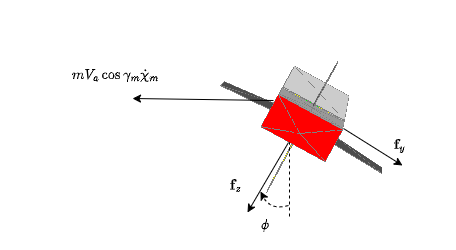
\includegraphics[width=0.49\linewidth]{./figures/vehicle_forces_lateral.png}
  		\caption{The lateral forces acting on the hypersonic vehicle when the course angle $\chi_m$ is changing.}
  	\label{fig:vehicle_forces_lateral}
  	\end{figure} 	
The lateral forces acting on the hypersonic vehicle are shown in Figure~\ref{fig:vehicle_forces_lateral}.  Summing the forces along the lateral axis gives
\[
mV_m \cos\gamma_m \dot{\chi}_m = f_z\sin\phi + f_y\cos\phi,
\]
from which we obtain
\[
\dot{\chi}_m = \frac{f_z\sin\phi + f_y\cos\phi}{mV_m\cos\gamma_m}.
\]

If we employ a roll stabilization loop that ensures that the roll angle $\phi=0$, then 
\begin{align*}
	\begin{pmatrix}	\dot{\chi}_m \\ \dot{\gamma}_m	\end{pmatrix}
	= \frac{1}{V_m}\begin{pmatrix} \frac{f_y}{m\cos\gamma_m} \\ g\cos\gamma_m + \frac{f_z}{m} \end{pmatrix}.
\end{align*}


Therefore
%\begin{align*}
%	\abf_{m/i}^\ell	= \begin{pmatrix}
%						
% 	
% 					   \end{pmatrix}
%\end{align*}

\section{Autopilot Design}

For all controllers, the maximum rudder deflection is 0.008 radians. Any commanded deflection greater than this is saturated.

The controller for roll is shown in Figure~\ref{fig:roll_control}. Note that for this application, $\phi^c$ is always equal to zero. A positive $\phi$ value refers to a roll to the right when looking down the nose of the missile. 

An anti-windup scheme is also used in that the integrator only updates when the absolute error is within 0.02 radians.

\begin{figure}[h!]
\centering
    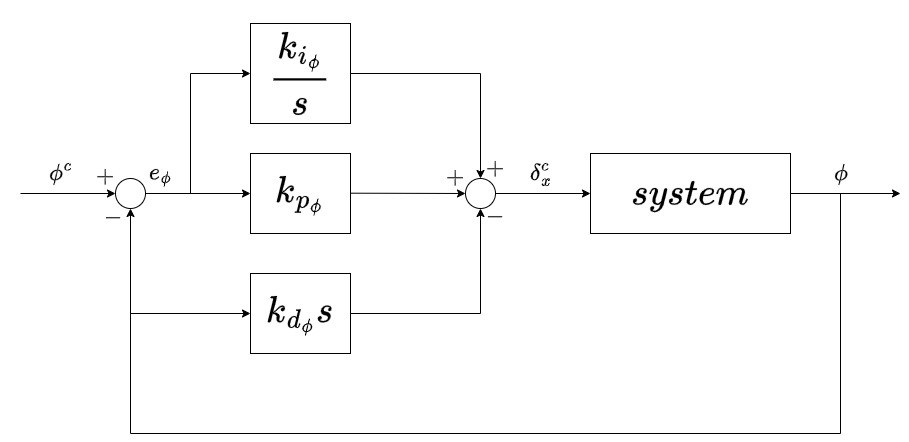
\includegraphics[width=1.0\linewidth]{./figures/roll_controller.drawio.png}
    \caption{Roll attitude control loop.}
    \label{fig:roll_control}
\end{figure} 

\FloatBarrier

The course controller is shown in Figure~\ref{fig:yaw_control}. A positive $\chi$ value refers to the clockwise angle from north when looking from a birds-eye view above the missile.

\begin{figure}[h!]
    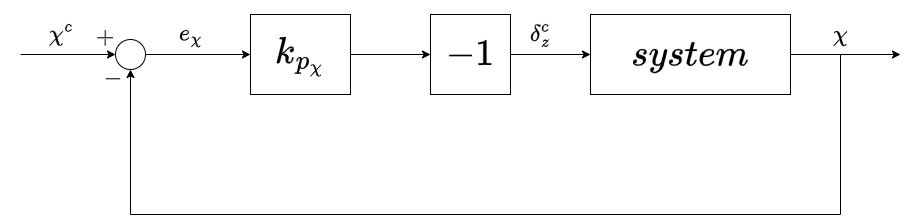
\includegraphics[width=1.0\linewidth]{./figures/course_controller.drawio.png}
    \caption{Course control loop.}
    \label{fig:yaw_control}
\end{figure} 

The autopilot for longitudinal control with successive loop closure is shown in Figure~\ref{fig:long_control}. The inner loop (shaded in gray) is the pitch controller (see Figure~\ref{fig:pitch_control}), and the outer loop is the altitude controller (see Figure~\ref{fig:altitude_control}).

\begin{figure}[h!]
    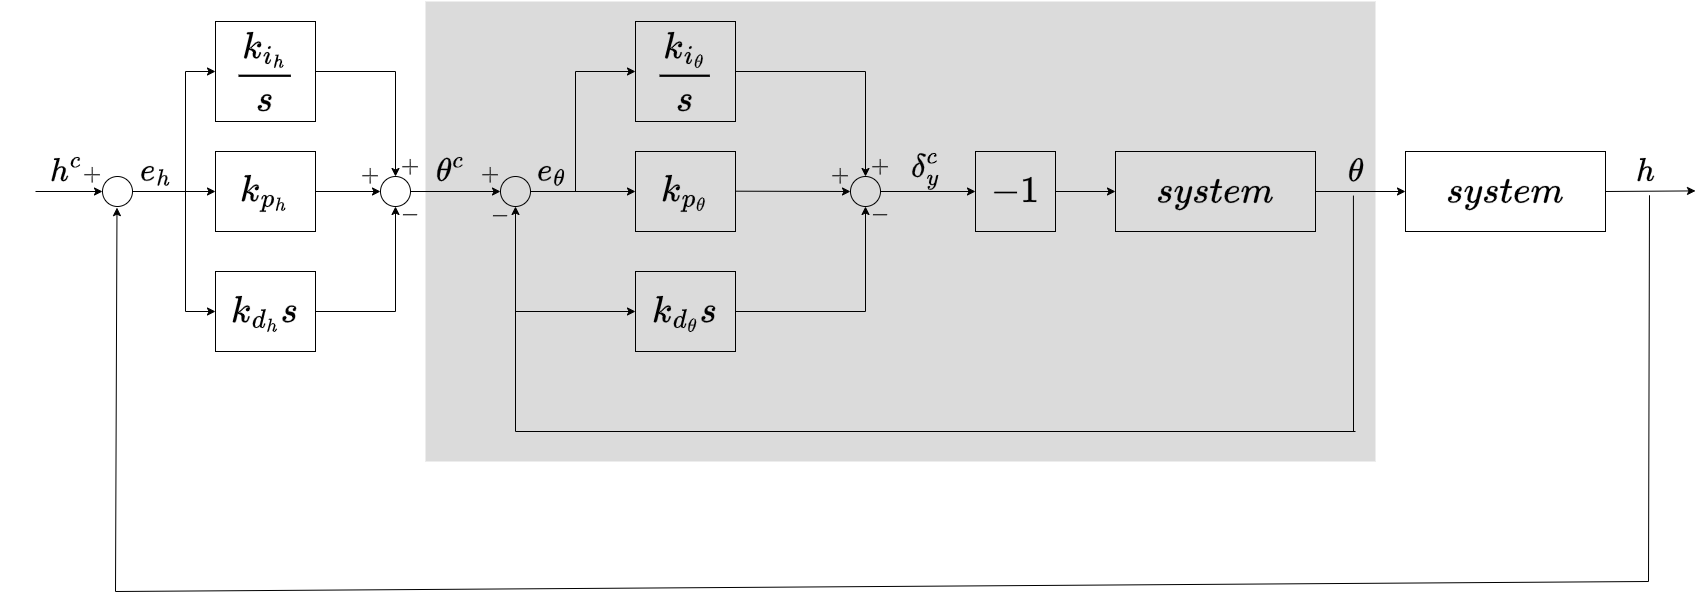
\includegraphics[width=1.0\linewidth]{./figures/longitudinal_controller.drawio.png}
    \caption{Autopilot for longitudinal control using successive loop closure.}
    \label{fig:long_control}
\end{figure}

\FloatBarrier

The pitch controller is set to saturate the commanded pitch at 90 degrees. It also incorporates an anti-windup scheme where the integrator only updates when the absolute value of the time derivative of the error is less than 0.01 m/s. This derivative is calculated as follows:

\begin{align*}
	\dot e[n] = \frac{2\sigma - T_s}{2\sigma + T_s}\dot e[n-1] + \frac{2}{2\sigma + T_s}(e[n] - e[n - 1])
\end{align*}

where $\sigma$ is a constant set at a value of 0.05.

\begin{figure}[h!]
    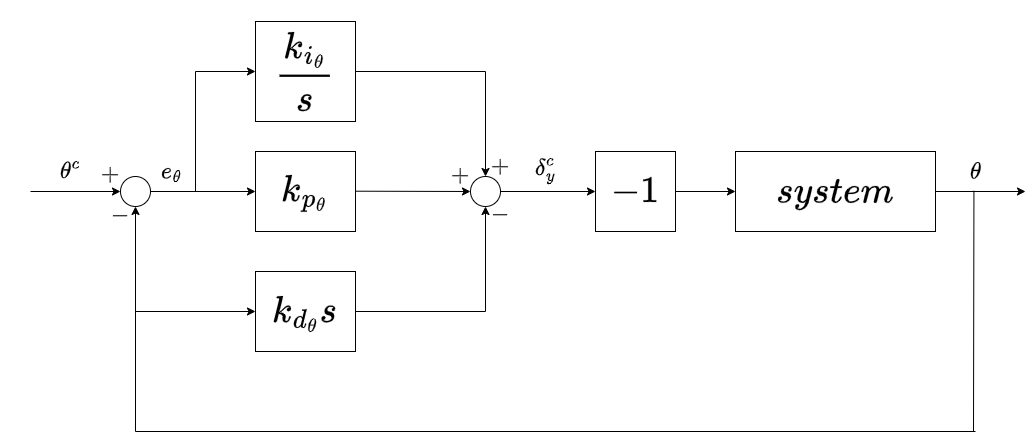
\includegraphics[width=1.0\linewidth]{./figures/pitch_controller.drawio.png}
    \caption{Pitch attitude control loop.}
    \label{fig:pitch_control}
\end{figure} 

\FloatBarrier
The altitude control loop in Figure~\ref{fig:altitude_control} approximates the inner loop with the DC gain $K_{\theta_{DC}}$. However, this gain was not explicitly calculated. Instead, an integral feedback term was employed to ensure unity DC gain on the inner loop, and empirical tests have shown that the resulting bandwidth of the inner loop does not limit performance with altitude control. \\
The integrator for the altitude controller also employs an anti-windup scheme where the integrator only updates when the absolute value of the time derivative of the error is less than 5 m/s.

\begin{figure}[h!]
    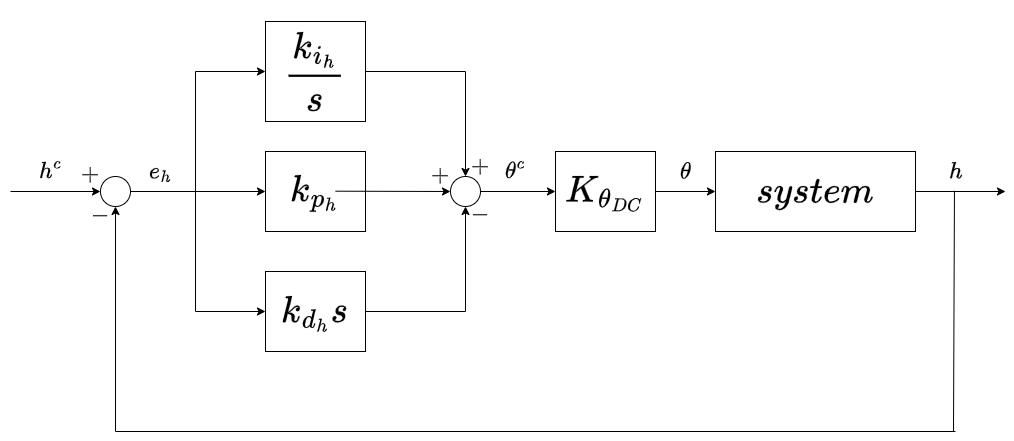
\includegraphics[width=1.0\linewidth]{./figures/altitude_controller.drawio.png}
    \caption{Altitude control loop.}
\label{fig:altitude_control}

\end{figure} 

\FloatBarrier

The selected gains for the autopilot are shown in Table~\ref{tab:autopilot_gains}.

\begin{table}[h!]
\caption{Autopilot gains.}
\centering
 \begin{tabular}{||c c||} 
 \hline
 Parameter & Value \\ [0.5ex] 
 \hline\hline
 $k_{p_\phi}$ & $0.004$\\ 
 $k_{i_\phi}$ & $0.001$\\
 $k_{d_\phi}$ & $0.002$\\
 $k_{p_\theta}$ & $0.2$\\
 $k_{i_\theta}$ & $0.2$\\
 $k_{d_\theta}$ & $0.005$\\
 $k_{p_\chi}$ & $0.08$\\
 $k_{p_h}$ & $0.0006$\\
 $k_{i_h}$ & $0.00001$\\
 $k_{d_h}$ & $0.0006$\\[1ex] 
 \hline
 \end{tabular}
 \label{tab:autopilot_gains}
\end{table}

\FloatBarrier
\bibliographystyle{IEEEtran}
\bibliography{library}
References go here.

\end{document}